%这个是根据计算机学报官网下的LaTeX模板改的，主要修改内容：①把GBK编码改成了UTF-8编码。②引入zhwinfonts，用上传的字体文件实现了字体的使用。
%现存的问题：①中文无法使用加粗功能，但是英文可以。解决方式1：使用黑体来凑合代替。解决方式2：在PDF编辑器里面一个一个加粗。②无法实现模板中所要求的每页脚注从1开始的要求。
%如果您在使用该模板的过程中遇到问题，或者有对该模板的修改意见，请联系本人：微信PolarisRisingWar（诸神缄默不语），或者CSDN诸神缄默不语（PolarisRisingWar）

\documentclass[10.5pt,compsoc]{CjC}
\usepackage{CJKutf8}
% \usepackage{CJK}
% \usepackage{xeCJK}
\usepackage{graphicx}
\usepackage{footmisc}
\usepackage{subfigure}
\usepackage{url}
\usepackage{multirow}
\usepackage[noadjust]{cite}
\usepackage{amsmath,amsthm}
\usepackage{amssymb,amsfonts}
\usepackage{booktabs}
\usepackage{color}
\usepackage{ccaption}
\usepackage{booktabs}
\usepackage{float}
\usepackage{fancyhdr}
\usepackage{caption}
\usepackage{xcolor,stfloats}
\usepackage{comment}
\setcounter{page}{1}
\graphicspath{{figures/}}
\usepackage{cuted}%flushend,
\usepackage{captionhack}
\usepackage{epstopdf}
\usepackage[utf8]{inputenc}
%\usepackage{ccmap}
%\CJKtilde
%\usepackage{CJKpunct} 
%\usepackage[lite,subscriptcorrection,slantedGreek,nofontinfo]{mtpro2}

% 伪代码宏包（此部分你可以加入）
\usepackage{algorithm}
\usepackage{algpseudocode}
\usepackage{svg}
\algrenewcommand\algorithmiccomment[1]{\hfill\textit{// #1}}

%===============================%

%\firstfootname{ \quad \quad }
\headevenname{\mbox{\quad} \hfill  \mbox{\zihao{-5}{\begin{CJK*}{UTF8}{song}计\quad \quad 算\quad \quad 机\quad \quad 学\quad \quad 报\end{CJK*}} \hspace {50mm} \mbox{\begin{CJK*}{UTF8}{song}2025 年\end{CJK*}}}}%
\headoddname{\begin{CJK*}{UTF8}{song}1 期 \hfill
作者姓名等：论文题目\end{CJK*}}%

%footnote use of *
\renewcommand{\thefootnote}{\fnsymbol{footnote}}
\setcounter{footnote}{0}
\renewcommand\footnotelayout{\zihao{5-}}

\newtheoremstyle{mystyle}{0pt}{0pt}{\normalfont}{1em}{\bf}{}{1em}{}
\theoremstyle{mystyle}
\renewcommand\figurename{figure~}
\renewcommand{\thesubfigure}{(\alph{subfigure})}
\newcommand{\upcite}[1]{\textsuperscript{\cite{#1}}}
\renewcommand{\labelenumi}{(\arabic{enumi})}
\newcommand{\tabincell}[2]{\begin{tabular}{@{}#1@{}}#2\end{tabular}}
\newcommand{\abc}{\color{white}\vrule width 2pt}
\makeatletter
\renewcommand{\@biblabel}[1]{[#1]\hfill}
\makeatother
\setlength\parindent{2em}
%\renewcommand{\hth}{\begin{CJK*}{UTF8}{zhhei}}
%\renewcommand{\htss}{\begin{CJK*}{UTF8}{song}}

\input{zhwinfonts}
\begin{document}
\hyphenpenalty=50000
\makeatletter
\newcommand\mysmall{\@setfontsize\mysmall{7}{9.5}}
\newenvironment{tablehere}
  {\def\@captype{table}}

\let\temp\footnote
\renewcommand \footnote[1]{\temp{\zihao{-5}#1}}


\thispagestyle{plain}%
\thispagestyle{empty}%
\pagestyle{CjCheadings}

\begin{table*}[!t]
\vspace {-13mm}
\begin{tabular}{p{168mm}}
\zihao{5-}\begin{CJK*}{UTF8}{song}
第1卷\quad 第1期 \hfill 计\quad 算\quad 机\quad 学\quad 报\hfill Vol. 1  No. 1\end{CJK*}\\
\zihao{5-}\begin{CJK*}{UTF8}{song}
2025年1月 \hfill CHINESE JOURNAL OF COMPUTERS \hfill 1. 2025\end{CJK*}\\
\hline\\[-4.5mm]
\hline\end{tabular}

\centering
\vspace {11mm}
\begin{CJK*}{UTF8}{zhhei}
{\zihao{2} 算法驱动的迷宫探险游戏开发方法 }
\end{CJK*}
\vskip 5mm

{\zihao{3}\begin{CJK*}{UTF8}{fs}
张佳栋\quad  方维 \quad 逯熙钰 \quad 姜舜航\end{CJK*}}

\vspace {5mm}
\zihao{6}{\begin{CJK*}{UTF8}{song}
(东北大学 计算机科学与工程学院 \quad 沈阳 \quad 110169)
\end{CJK*}}

% \zihao{6}{\begin{CJK*}{UTF8}{song}
% $^{1)}$(单位全名 部门(系)全名, 市(或直辖市) 国家名 邮政编码)
% *字体为6号宋体*单位
% \end{CJK*}}

% \zihao{6}{\begin{CJK*}{UTF8}{song}
% $^{2)}$(单位全名 部门(系)全名, 市(或直辖市) 国家名
% 邮政编码)*中英文单位名称、作者姓名须一致*
% \end{CJK*}}

% \zihao{6}{\begin{CJK*}{UTF8}{song}
% $^{3)}$(单位全名 部门(系)全名, 市(或直辖市) 国家名 邮政编码)
% \end{CJK*}}

% \zihao{6}{\begin{CJK*}{UTF8}{zhhei}
% 论文定稿后，作者署名、单位无特殊情况不能变更。若变更，须提交签章申请，国家名为中国可以不写，省会城市不写省的名称，其他国家必须写国家名。
% \end{CJK*}}

\vskip 5mm
{\centering
\begin{tabular}{p{160mm}}
\zihao{5-}{
\setlength{\baselineskip}{16pt}\selectfont{
\noindent\begin{CJK*}{UTF8}{zhhei}摘\quad 要\quad \end{CJK*} \begin{CJK*}{UTF8}{song}
本文提出了一种融合经典算法策略的迷宫探险游戏开发方法, 
涵盖从迷宫生成到智能策略执行的完整流程.
首先, 基于分治法生成满足"无孤立区域存在唯一通路"的随机迷宫,
支持多种尺寸, 并实现了游戏过程的~\textrm{OpenGL}~动态可视化.
其次, 采用树形动态规划实现全局资源收集路径规划,
确保在避开陷阱的前提下最大化资源总值;
实验中, 该方法在~$100$~组~$7 \times 7$~迷宫中的平均资源得分为~$6.72$. 
针对有限视野场景, 设计了一种贪心策略和启发式策略, 
通过预期收益函数实现局部最优选择, 平均得分达~$6.18$, 
较普通贪心策略~($4.89$)~提高~$26.3\%$.
此外, 利用回溯法构建密码解谜系统, 在限制条件下成功解出所有3位数谜题;
在~$\textrm{BOSS}$~战斗模块中, 基于分支限界法实现技能序列优化策略,
在可用资源有限的情况下稳定输出最小回合击败序列.
整体框架展示了各类算法在路径规划、决策优化和策略推理中的有效结合,
为算法驱动的游戏开发提供了实用范式.

\end{CJK*}\par}}\\[2mm]

\zihao{5-}{\noindent
\begin{CJK*}{UTF8}{zhhei}关键词\end{CJK*} \quad \begin{CJK*}{UTF8}{song}{迷宫生成; 树形~$\textrm{DP}$; 贪心策略; 启发式策略; 回溯法; 分支限界法; 可视化}
% \begin{CJK*}{UTF8}{zhhei}关键词\end{CJK*} \quad \begin{CJK*}{UTF8}{song}{*关键词（中文关键字与英文关键字对应且一致，应有5-7个关键词)；关键词；关键词；关键词*  }
\end{CJK*}
}\\[2mm]
\zihao{5-}{\begin{CJK*}{UTF8}{zhhei}中图法分类号\end{CJK*}	\begin{CJK*}{UTF8}{song}
TP\end{CJK*}\rm{\quad \quad \quad     }}
\end{tabular}}

\vskip 7mm

\begin{center}
\zihao{3}{ {\begin{CJK*}{UTF8}{zhhei}Algorithm-Driven Maze Exploration Game Development Method\end{CJK*}}}\\
\vspace {5mm}
\zihao{5}{ {\begin{CJK*}{UTF8}{zhhei}ZHANG Jia-Dong \quad FANG Wei \quad LU Xi-Yu \quad JIANG Shun-Hang\end{CJK*}
}}\\
\vspace {2mm}
\zihao{6}{\begin{CJK*}{UTF8}{zhhei}{(School of Computer Science and Engineering, Northeastern University, Shenyang 110169, China)}\end{CJK*}}

% \zihao{6}{\begin{CJK*}{UTF8}{zhhei}{$^{1)}$(Department of ****, University, City ZipCode, China) *字体为6号Times
% new Roman* Depart.Correspond}\end{CJK*}}

% \zihao{6}{\begin{CJK*}{UTF8}{zhhei}{$^{2)}$(Department of ****, University, City ZipCode)*中国不写国家名*}\end{CJK*}}

% \zihao{6}{\begin{CJK*}{UTF8}{zhhei}{$^{3)}$(Department of ****, University, City ZipCode, country)*外国写国家名*}\end{CJK*}}



\end{center}

\begin{tabular}{p{160mm}}
\zihao{5}{
\setlength{\baselineskip}{18pt}\selectfont{
{\bf Abstract}\quad \begin{CJK*}{UTF8}{zhhei}
This paper presents a maze exploration game development framework integrating classical algorithmic strategies, covering the entire process from maze generation to intelligent strategy execution.
First, a divide-and-conquer approach is used to generate random mazes that guarantee unique solvable paths without isolated regions. The system supports multiple maze sizes and features real-time OpenGL-based visualization.
Second, a tree-based dynamic programming method is adopted for global resource collection path planning, ensuring maximum total value while avoiding traps.
In experiments on $100$ randomly generated $7 \times 7$ mazes, this method achieved an average resource score of $6.72\%$.
For limited-vision scenarios, both a greedy strategy and a heuristic strategy are designed. A reward expectation function guides local optimal selection, resulting in an average score of $6.18$ with an improvement of $26.3\%$ over the basic greedy approach ($4.89$).
Additionally, a backtracking algorithm is employed to construct a password puzzle system, successfully solving all 3-digit puzzles under given constraints.
In the boss battle module, a branch-and-bound method is used to optimize the skill sequence, consistently generating minimal-turn victory strategies under limited player resources.
This framework demonstrates an effective integration of various algorithms in path planning, decision-making, and strategic reasoning, offering a practical paradigm for algorithm-driven game development.
\end{CJK*}
\par}}\\

\setlength{\baselineskip}{18pt}\selectfont{
\zihao{5}{
  
% \vspace {5mm}
{\bf Keywords}\quad \begin{CJK*}{UTF8}{zhhei}
maze generation; tree-based DP; greedy strategy; heuristic strategy; backtracking; branch and bound; visualization
\end{CJK*}}\par}
\end{tabular}

\setlength{\tabcolsep}{2pt}
\begin{tabular}{p{0.05cm}p{16.15cm}}
% \multicolumn{2}{l}{\rule[4mm]{40mm}{0.1mm}}\\[-3mm]
&\begin{CJK*}{UTF8}{song}
% 收稿日期：\quad \quad -\quad -\quad ；最终修改稿收到日期：\quad \quad -\quad -\quad .*投稿时不填写此项*. 本课题得到… …基金中文完整名称(No.项目号)、… …基金中文完整名称(No.项目号)、… … 基金中文完整名称(No.项目号)资助.作者名1(通信作者)，性别，xxxx年生，学位(或目前学历)，职称，是/否计算机学会(CCF)会员（提供会员号),主要研究领域为*****、****.E-mail: **************.作者名2（通信作者)，性别，xxxx年生，学位(或目前学历)，职称，是/否计算机学会(CCF)会员（提供会员号),主要研究领域为*****、****.E-mail: **************. 作者名3（通信作者)，性别，xxxx年生，学位(或目前学历)，职称，是/否计算机学会(CCF)会员（提供会员号),主要研究领域为*****、****.E-mail: **************.(给出的电子邮件地址应不会因出国、毕业、更换工作单位等原因而变动。请给出所有作者的电子邮件)
% 第1作者手机号码(投稿时必须提供，以便紧急联系，发表时会删除): … …, E-mail: … …*此部分6号宋体*
\end{CJK*}
\end{tabular}\end{table*}
\clearpage\clearpage
\begin{strip}
\vspace {-13mm}
\end{strip}
\linespread{1.15}

\begin{CJK*}{UTF8}{zhhei}
\zihao{5}
\vskip 1mm
\section{项目概述}
\end{CJK*}

\begin{CJK*}{UTF8}{song}
本项目旨在开发一款融合经典算法与图形可视化的迷宫探险游戏. 
通过将分治、动态规划、贪心、回溯、分支限界等算法设计策略贯穿于迷宫生成、资源收集、谜题解锁、战斗系统等多个关键模块,
实现算法理论与工程实践的深度融合.

项目主要有以下模块:

(1) 分治法生成随机迷宫

(2) 动态规划求解最优资源收集路径

(3) 贪心算法实时策略模拟

(4) 启发式算法实时策略模拟

(5) 回溯法解锁机关密码

(6) 分支限界法优化~$\textrm{BOSS}$~战斗策略

(7) 基于~$\textrm{OpenGL}$~的可视化演示
\end{CJK*}

\begin{CJK*}{UTF8}{zhhei}
\zihao{5}
\vskip 1mm
\section{分治法地图生成}
\end{CJK*}


\begin{CJK*}{UTF8}{zhhei}\subsection{问题描述}\end{CJK*}

\begin{CJK*}{UTF8}{song}
任务: 使用分治法生成迷宫, 无孤立区域, 存在唯一通路.

输入: 迷宫尺寸.

输出: 迷宫矩阵~(可存储为~JSON~或~CSV), 包括起点~Start(S)、
终点~Exit(E)、墙壁~(\#)、通路~(空格)、资源~(例如金币~G)、
陷阱~Trap(T)、机关~Locker(L)、BOSS(B).
\end{CJK*}

\begin{CJK*}{UTF8}{zhhei}\subsection{算法设计}\end{CJK*}

\begin{CJK*}{UTF8}{song}
\begin{CJK*}{UTF8}{zhhei}{1. 初始化迷宫}\end{CJK*}

创建二维数组表示迷宫, 尺寸为奇数~(如~$\textrm{height} \times \textrm{width}$).

\begin{CJK*}{UTF8}{zhhei}{2. 递归分割区域}\end{CJK*}

输入参数: 子问题迷宫的左上方坐标和右下方坐标.

终止条件: 区域宽度或高度小于~$2$.

\begin{CJK*}{UTF8}{zhhei}{3. 选择分割方向}\end{CJK*}

随机选择一个纵向墙体 (非外围) 和一个横向墙体 (非外围), 视其把迷宫分割为四个部分作为其子问题并求解,
同时在四片墙体中随机选取三个墙体将其打通, 由于~$2 \times 2$ 迷宫的特殊性,
这样生成的迷宫路径唯一且无环路, 且无需合并子问题$^{[1]}$.

\begin{CJK*}{UTF8}{zhhei}{4. 设置入口和出口}\end{CJK*}

入口：在迷宫最外围墙体 (非四个角) 上随机选择一个作为入口.

出口：在迷宫最外围墙体 (非四个角) 上随机选择一个作为出口, 若与出口重合, 则重新生成直到不同.

\begin{CJK*}{UTF8}{zhhei}{5. 添加资源和陷阱}\end{CJK*}

随机在迷宫中添加资源和陷阱, 数量和位置可根据需求设定.
\end{CJK*}

\begin{CJK*}{UTF8}{zhhei}\subsection{复杂度分析}\end{CJK*}

\begin{CJK*}{UTF8}{song}
下面用归纳法证明对于生成一个~$a \times b$~的迷宫的时间复杂度是~$\mathcal{O}(a \times b)$.

由于最小子问题是一个~$1 \times n$~或~$n \times 1$~大小的块, 
处理这样一个子问题的复杂度是~$\mathcal{O}(n)$~的, 满足归纳假设.

假设对于所有~$a < A, b < B$~的问题的复杂度~$T(a,b) = \mathcal{O}(a \times b)$.

对于一个~$A \times B$~的问题, 假设划分大小为~$p, q$. 划分的复杂度为~$\mathcal{O}(1)$.

那么复杂度

\vskip -4mm

\begin{align*}
T(A,B) &= \mathcal{O}(1) + T(p,q) + T(p,B-q) + {} \\
       &\quad + T(A-p,q) + T(A-p,B-q) \\
       &= \mathcal{O}(1) + \mathcal{O}(p \times q) + \mathcal{O}(p \times (B - q)) + {} \\
       &\quad + \mathcal{O}((A - p) \times q) + \mathcal{O}((A - p) \times (B - q)) \\
       &= \mathcal{O}(A \times B).
\end{align*}


所以, 规模为~$a \times b$~的问题的时间复杂度是~$\mathcal{O}(a \times b)$.

特别的, 当~$a=b=n$~时, 复杂度为~$\mathcal{O}(n^2)$.
\end{CJK*}

\begin{CJK*}{UTF8}{zhhei}\subsection{伪代码}\end{CJK*}

\begin{CJK*}{UTF8}{song}
见附录~1.
\end{CJK*}

% @DP

\begin{CJK*}{UTF8}{zhhei}
\zihao{5}
\vskip 1mm
\section{动态规划求解最优路径}
\end{CJK*}


\begin{CJK*}{UTF8}{zhhei}\subsection{问题描述}\end{CJK*}

\begin{CJK*}{UTF8}{song}
任务: 计算从起点到终点的最优资源收集路径, 避开陷阱, 优先拾取资源.
例如: 状态~dp[i][j]~表示走到坐标(i,j)时的最大资源值.

输入：迷宫矩阵、资源分布 (例如金币~$=5$)、陷阱位置 (可设置陷阱~$=-3$).

输出: 最大资源值、最优路径序列.

需求: 路径可视化 (可选).

\begin{CJK*}{UTF8}{zhhei}\subsection{问题分析}\end{CJK*}

目标: 从迷宫的起点出发, 到达终点, 经过必须经过的机关和~BOSS, 收集最多的资源.

分析: 地图保证了路径唯一, 可知地图实际是一个树形结构, 可以采用树形~DP$^{[5]}$.
我们以起点为根, 构建地图对应的树.
问题就转化为了有一颗带权树, 要求找一条从根到终点的通路, 使得通路上的权值和最大$^{[2]}$.


\begin{CJK*}{UTF8}{zhhei}\subsection{状态设计及状态转移方程}\end{CJK*}

定义~$\textrm{dp}_{i, j}$~表示从点~$(i,j)$~出发能获得的最大价值,
$\textrm{must}_{i,j}$~表示点~$(i,j)$~是否为从起点到终点必须经过的点.
那么答案即为~$\textrm{dp}_s$, 其中~$s$~为起点的坐标.
那么有转移方程：

\begin{align*}
\textrm{must}_p = 
\begin{cases}
\displaystyle \bigvee_{x\in{\text{son}}_p} \textrm{must}_x, & \text{if } x \text{ is not E} \\
1, & \text{if } x = \text{is E} \\
\end{cases}
\end{align*}

\begin{align*}
\textrm{dp}_p = w_p + \displaystyle \sum_{x\in{\text{son}}_p}
\begin{cases}
\textrm{dp}_x, & \text{if } \textrm{must}_x \\
\max(\textrm{dp}_x, 0), & \text{else} \\
\end{cases}
\end{align*}


\begin{CJK*}{UTF8}{zhhei}\subsection{最优路径构建}\end{CJK*}

对于不同~$\textrm{must}$~的点的构建方法不同.

对于~$\textrm{must}$~为真的节点, 需要先输出自己的坐标,
然后依次构建~$\textrm{must}$~为假并且采用其中权值的子树的路径,
中间穿插自己的坐标, 最后构建~$\textrm{must}$~为真的子树的路径.

对于~$\textrm{must}$~为假的节点, 也需要先输出自己的坐标,
然后依次构建采用其中权值的子树的路径, 中间穿插自己的坐标,
并且最后也要输出自己的坐标.

% \end{CJK*}

\begin{figure}[htbp]
\centerline{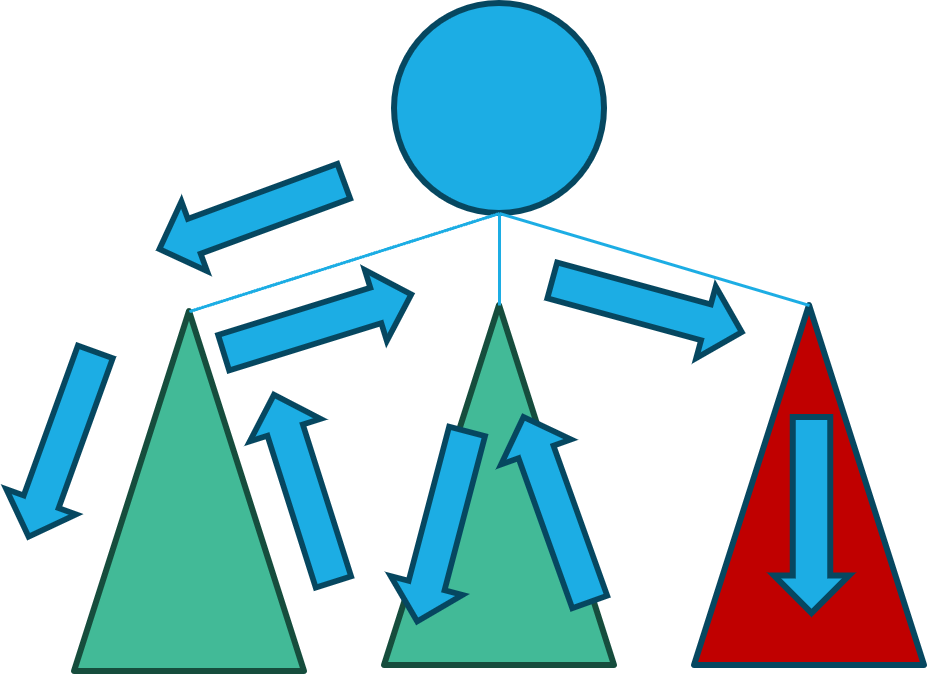
\includegraphics[width=3in]{./figure/fig1.png}}
\begin{CJK*}{UTF8}{song}图1\quad  $\textrm{must}$~为真的节点的子树路径构建顺序\end{CJK*}
\label{fig1}
\end{figure}

\begin{figure}[htbp]
\centerline{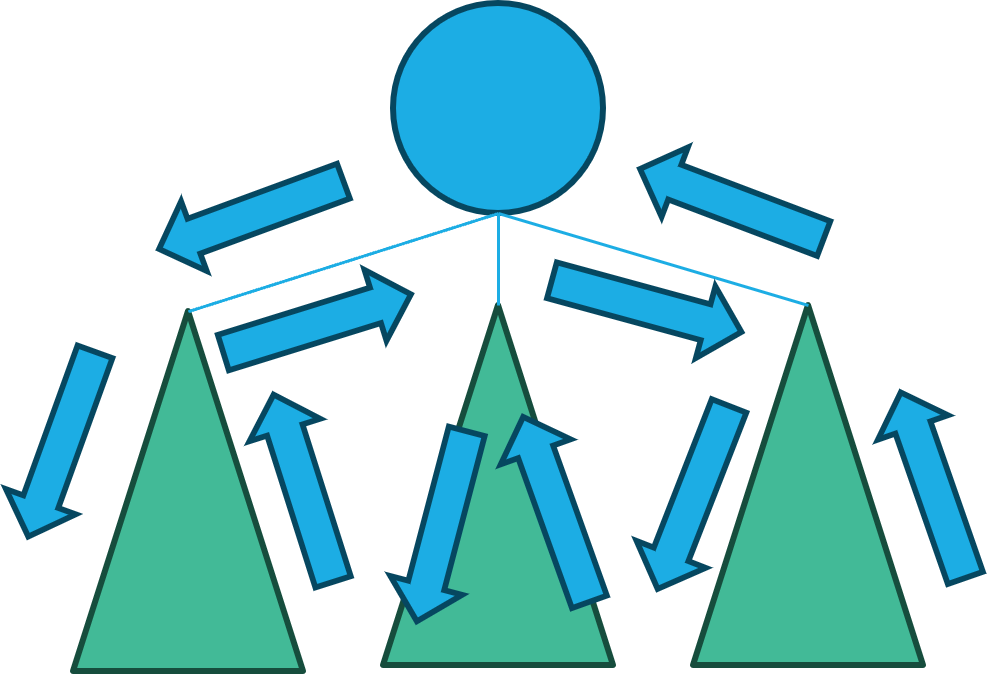
\includegraphics[width=3.15in]{./figure/fig2.png}}
\begin{CJK*}{UTF8}{song}图2\quad  $\textrm{must}$~为假的节点的子树的路径构建顺序\end{CJK*}
\label{fig2}
\end{figure}


\begin{CJK*}{UTF8}{zhhei}\subsection{复杂度分析}\end{CJK*}


本算法采用自底向上的树形动态规划方法,
其中每个点~$p$~只会在其父节点的转移中被访问一次,
而~$\textrm{must}$~的计算也是在一次~DFS~遍历中完成的.

首先, 自底向上计算每个点是否为必须经过的点, 即~$\textrm{must}_p$.
该过程为一次~DFS, 遍历所有点与边, 时间复杂度为~$\mathcal{O}(n)$.

接下来计算每个点的~$\textrm{dp}_p$,
其依赖于所有子节点的~$\textrm{dp}_x$.
由于每条边最多只会被访问一次, 整个~DP~的计算同样是~$\mathcal{O}(n)$.

因此, 总体时间复杂度为: 
\[
\mathcal{O}(n + m)
\]

该算法空间复杂度也为~$\mathcal{O}(n)$,
用于记录每个点的~$\textrm{dp}$~和~$\textrm{must}$~状态.

\begin{CJK*}{UTF8}{zhhei}\subsection{伪代码}\end{CJK*}

% \begin{CJK*}{UTF8}{song}

见附录~1.

\end{CJK*}


% @贪心
\begin{CJK*}{UTF8}{zhhei}
\zihao{5}
\vskip 1mm
\section{贪心算法实时策略模拟}
\end{CJK*}

\begin{CJK*}{UTF8}{song}
    
\begin{CJK*}{UTF8}{zhhei}\subsection{问题描述}\end{CJK*}

任务: 玩家视野受限于周围区域, 每次移动时优先选择视野内~"性价比"(例如单位距离收益最大) 最高的资源, 重复直至无资源可拾取.
输入: 当前玩家位置、视野内的资源信息.
输出: 资源拾取路径.
    
\begin{CJK*}{UTF8}{zhhei}\subsection{贪心策略}\end{CJK*}

\begin{CJK*}{UTF8}{zhhei}1. 优先级驱动的贪心算法\end{CJK*}

分四个优先级搜索目标, 优先级为:

\vskip -4.5mm
$$
\textrm{BOSS~/~机关} > \textrm{金币} > \textrm{通路} > \textrm{出口}.
$$

每个阶段只考虑当前最高优先级的可行目标.

\begin{CJK*}{UTF8}{zhhei}2. 记忆已探索地图\end{CJK*}

维持视野为~$3 \times 3$~范围, 但记录已探索的区域.
利于收集暂时被搁置的资源, 探索待探索的区域.
动态更新环境认知, 优先利用已知信息, 逐步扩展未知区域.

\begin{CJK*}{UTF8}{zhhei}3. 贪心探索路径\end{CJK*}

优先尝试非陷阱路径,
失败后才降级允许陷阱路径,
当高优先级目标不可达时, 会降级搜索低优先级目标.
    
\begin{CJK*}{UTF8}{zhhei}\subsection{复杂度分析}\end{CJK*}

在最坏情况下, 可能需要探索整个地图遍历所有~$n^2$~个格子.
每次寻找当前最高优先级的目标, 可以使用一个大根堆,
取得一次最高优先级的元素复杂度为~$\mathcal{O}(\log (n^2)) = \mathcal{O}(\log n)$.
所以总的时间复杂度为~$\mathcal{O}(n^2 \log n)$.
    
\begin{CJK*}{UTF8}{zhhei}\subsection{伪代码}\end{CJK*}

见附录~1.

\end{CJK*}


% @启发式
\begin{CJK*}{UTF8}{zhhei}
\zihao{5}
\vskip 1mm
\section{启发式算法实时策略模拟}
\end{CJK*}

\begin{CJK*}{UTF8}{song}
    
\begin{CJK*}{UTF8}{zhhei}\subsection{原有算法的不足和改进}\end{CJK*}

原本的贪心算法虽然可以找到一个尽可能最大化资源且符合要求的路径,
但是有些情况下, 它会被陷阱“吓到”而损失了金币,
毕竟谁也不知道一个陷阱的背后是另一块陷阱还是一大片金币.
换而言之, 原本的贪心算法十分“保守”.

对此, 我们提出了一种启发式的算法,
该算法在原有贪心的基础上, 引入了估价函数,
对于一片被陷阱挡住的未知区域, 我们可以计算其期望的价值来判断是否“冒险”进入.

    
\begin{CJK*}{UTF8}{zhhei}\subsection{算法描述}\end{CJK*}

为了实现以上改进, 我们优化后的算法有以下几个部分组成:

1. 视野更新机制

2. 优先级策略设计~(策略核心)

3. 预期资源收益估计

\subsubsection{视野更新机制}

只更新当前位置周围~$3 \times 3$~的格子,未探索区域标记为未知.
每当角色移动到新位置, 就拓展一圈视野, 更新地图.

\subsubsection{优先级策略设计~(策略核心)}

核心目标: 在已知有限信息下, 选择最“有希望”的方向前进.

在没有找全~BOSS~和机关的情况下:
$$
\textrm{金币}=\textrm{通路}=\textrm{BOSS}=\textrm{机关}>\textrm{陷阱}>\textrm{终点}.
$$

在找全~BOSS~和机关的情况下:
$$
\textrm{金币}=\textrm{通路}=\textrm{BOSS}=\textrm{机关}>\textrm{陷阱}>\textrm{终点}.
$$

对于找全~BOSS~和机关的情况下如果可见且未到达方块中只有陷阱和终点,
我们需要计算陷阱和终点的预期资源收益估计, 如果一个陷阱的预期资源收益估计为正,
我们就会选择去“探索”.

\subsubsection{预期资源收益估计}

使用类似启发式扩展的方法, 预测从某个点出发能收集多少资源:
可见格子收益为 $1$ 倍；
未知格子按经验折扣估值, 乘一个系数~$r$.

\begin{CJK*}{UTF8}{zhhei}\subsection{复杂度分析}\end{CJK*}

在最坏情况下, 可能需要探索整个地图遍历所有~$n^2$~个格子.
每次寻找当前最高优先级的目标, 但是由于现在的优先级是实时更新的,不可以用大根堆,
所以取得一次最高优先级的元素复杂度为~$\mathcal{O}(n^2)$.
所以总的时间复杂度为~$\mathcal{O}(n^4)$.
    
\begin{CJK*}{UTF8}{zhhei}\subsection{实验结果}\end{CJK*}

对于~DP,~贪心,~启发式算法在随机生成的~100~个地图下测试, 计算平均收益.
\vskip 30mm

\begin{table}[htbp]
\centering {\begin{CJK*}{UTF8}{zhhei}表1\quad 各算法在不同地图规模下的执行效果比较\end{CJK*}} % 黑体表说明
\vspace{-2.5mm}
\begin{center}
\begin{tabular}{lccc}
\toprule
算法 & $7\times7$ & $11 \times 11$ & $15 \times 15$ \\  % 表头
\hline
贪心策略 & 85.3 & 78.2 & 65.4 \\
动态规划 & 89.1 & 83.7 & 71.8 \\
启发式算法 & 92.0 & 85.5 & 69.2 \\
\bottomrule
\end{tabular}
\label{tab1}
\end{center}
\end{table}
DP 得分最高: 由于拥有全图信息, 它能保证路径最优;

贪心策略表现最差: 虽快速但容易落入局部最优;

启发式方法综合表现优秀: 仅凭有限视野,
得分接近全图最优解,展现出“预期收益评估~+~策略优先级”的强大决策能力.

\end{CJK*}


% @回溯法
\begin{CJK*}{UTF8}{zhhei}
\zihao{5}
\vskip 1mm
\section{回溯法解锁机关密码}
\end{CJK*}

\begin{CJK*}{UTF8}{song}
\begin{CJK*}{UTF8}{zhhei}\subsection{问题描述}\end{CJK*}

输入: 一个~$3$~位密码锁的位置和线索 (如每位密码为素数且不重复、或第~$1$~位是偶数等)

输出: 密码

\begin{CJK*}{UTF8}{zhhei}\subsection{回溯法与剪枝策略}\end{CJK*}

本算法使用回溯法穷举所有三位密码组合,
并通过线索进行剪枝优化, 显著减少无效搜索空间$^{[3]}$.

剪枝函数判断当前构造出的密码是否满足全部线索条件:
\begin{itemize}
  \item 若线索为 \texttt{[-1, -1]}, 表示密码需为三位不同的素数;
  \item 若线索长度为 $2$, 如~\texttt{[1, 0]}~表示第~$1$~位必须为偶数;
  \item 若线索长度为 $3$, 如~\texttt{[5, -1, 3]}, 表示第~$1$~位为~$5$, 第~$3$~位为~$3$.
\end{itemize}

在回溯函数中, 每填一位数字即调用剪枝函数, 避免无效状态扩展.


\begin{CJK*}{UTF8}{zhhei}\subsection{复杂度分析}\end{CJK*}

最坏情况下, 尝试所有~$10^3 = 1000$~个三位数,
但在有效剪枝下, 实际遍历节点数远小于~$1000$, 记为~$T$.

对于每个状态调用一次剪枝函数, 每次最多遍历~$|C|$~条线索, 故总复杂度为:

\[
\mathcal{O}(T \cdot |C|)
\]

其中~$|C|$~为线索数, $T$ 通常远小于~$1000$.

\end{CJK*}


% @分支限界法
\begin{CJK*}{UTF8}{zhhei}
\zihao{5}
\vskip 1mm
\section{分支限界法优化~BOSS~战斗策略}
\end{CJK*}

\begin{CJK*}{UTF8}{song}
\begin{CJK*}{UTF8}{zhhei}\subsection{问题描述}\end{CJK*}

任务: 在限定回合内击败~BOSS, 寻找最小代价的技能序列.

输入: 玩家剩余资源、BOSS~血量、玩家可用技能 (例如, 普通攻击: 伤害5、无冷却; 
大招: 伤害10, 冷却2回合).

输出: 最小回合数的技能序列.

\begin{CJK*}{UTF8}{zhhei}\subsection{分支限界法与剪枝策略}\end{CJK*}

本策略用于规划击败多个~BOSS~的最优技能施放序列$^{[4]}$,
采用分支限界~(Branch and Bound)~法进行搜索.
每个状态包括：

\begin{itemize}
  \item 当前~BOSS~的血量数组;
  \item 当前正在攻击的~BOSS~编号;
  \item 当前时间步数~(回合);
  \item 各技能冷却状态;
  \item 技能使用历史序列.
\end{itemize}

通过启发式函数~\texttt{lowerBound}~
估计当前状态的最优代价下界~$bound = \texttt{turn} + \texttt{lowerBound}$,
若该值不优于当前最优解则立即剪枝. 
估价函数如下: 

\[
\texttt{lowerBound} = \left\lceil \frac{\text{剩余所有~BOSS~总血量}}{\text{平均每回合伤害}} \right\rceil
\]

同时, 为避免状态重复, 使用哈希函数记录已访问状态~\texttt{hashState},
并通过集合去重.


\begin{CJK*}{UTF8}{zhhei}\subsection{复杂度分析}\end{CJK*}

设~BOSS~数量为~$n$, 技能数量为~$k$, 最大每个~BOSS~血量为~$H$.

最坏情况下, 每一步可以选择~$k$~个技能或跳过, 最多打掉 $nH$ 点血, 理论状态空间为:

\[
\mathcal{O}(k^{nH}).
\]

但由于: 

\begin{itemize}
  \item 使用了优先队列, 每次优先扩展估价低的状态;
  \item 使用了估价剪枝, 大量不优路径被舍弃;
  \item 使用状态去重, 避免重复搜索;
\end{itemize}

因此实际状态扩展远少于指数级, 时间复杂度为:

\[
\mathcal{O}(T \cdot k)
\]

\vskip 10mm

其中~$T$~为实际扩展的状态数.

\end{CJK*}


% @结论
\begin{CJK*}{UTF8}{zhhei}
\zihao{5}
\vskip 1mm
\section{结论}
\end{CJK*}

\begin{CJK*}{UTF8}{song}

本文从多个维度探索了经典算法在迷宫探险游戏中的集成应用与落地实现.
通过构建满足特定可达性要求的迷宫生成器,
结合~\textrm{OpenGL}~动态可视化技术,
系统完成了从环境构造到交互展示的闭环.

在策略层面, 设计并实现了针对全局与局部视野的路径规划方案.
全局阶段采用动态规划算法, 有效规避陷阱并最大化资源收益;
局部阶段则结合贪心与启发式策略, 使智能体在不完全信息下作出高收益决策,
实验验证表明本方法在平均得分与稳定性上优于传统贪心策略.


同时, 针对游戏中的逻辑推理与战斗博弈模块, 分别引入回溯法与分支限界法,
成功实现对密码谜题的有效求解与~$\textrm{BOSS}$~战斗回合数的全局最优控制.
两者均利用剪枝策略显著降低搜索空间, 提升求解效率与实用性.

综上所述, 本文提出的算法融合式游戏设计模式不仅具备良好的通用性与可扩展性,
也为算法教学与智能体训练提供了有价值的范式示例.

\end{CJK*}

\begin{CJK*}{UTF8}{song}

% {\begin{CJK*}{UTF8}{zhhei}\subsection{二级标题 *字体为5号黑体*标题2}\end{CJK*}}
% \subsubsection{三级标题 *字体为5号宋体*标题3}
% *正文部分, 字体为5号宋体* 正文文字

% \textbf{正文文字要求语句通顺，无语法错误，结构合理，条理清楚，不影响审稿人、读者阅读理解全文内容。以下几类问题请作者们特别注意}：

% 1) 文章题目应明确反映文章的思想和方法；文字流畅，表述清楚；

% 2) 中文文字、英文表达无语法错误；

% 3) 公式中无符号、表达式的疏漏，没有同一个符号表示两种意思的情况；

% 4) 数学中使用的符号、函数名用斜体；

% 5) 使用的量符合法定计量单位标准；

% 6) 矢量为黑体，标量为白体；

% 7) 变量或表示变化的量用斜体；

% 8) 图表规范，量、线、序无误，位置正确(图表必须在正文中有所表述后出现，即{\ldots}如图1所示)(注意纵、横坐标应有坐标名称和刻度值)。

% 9) 列出的参考文献必须在文中按顺序引用，即参考文献顺序与引用顺序一致，各项信息齐全(格式见参考文献部分)；

% 10) 首次出现的缩写需写明全称，首次出现的符号需作出解释。

% 11) 图的图例说明、坐标说明全部用中文或量符号。

% \textbf{12) 图应为矢量图。}

% 13) 表中表头文字采用中文。

% 14) 公式尺寸：

% 标准：10.5磅

% 下标/上标：5.8磅

% 次下标/上标：4.5磅

% 符号：16磅

% 次符号：10.5磅

% 15) 组合单位采用标准格式，如：``pJ/bit/m$^{4}$''应为 ``pJ/(bit$\cdot
% $m$^{4})$''

% {\begin{CJK*}{UTF8}{zhhei}\textbf{定理1}.\end{CJK*}}\quad ******. *定理内容.*

% [``定义''、``假设''、``公理''、``引理''等的排版格式与此相同，详细定理证明、公式可放在附录中]

% {\begin{CJK*}{UTF8}{song}证明\end{CJK*}}.\quad  *证明过程.* [``例 x''等的排版格式相同]

% \rightline {证毕.}

% \begin{figure}[htbp]
% \centerline{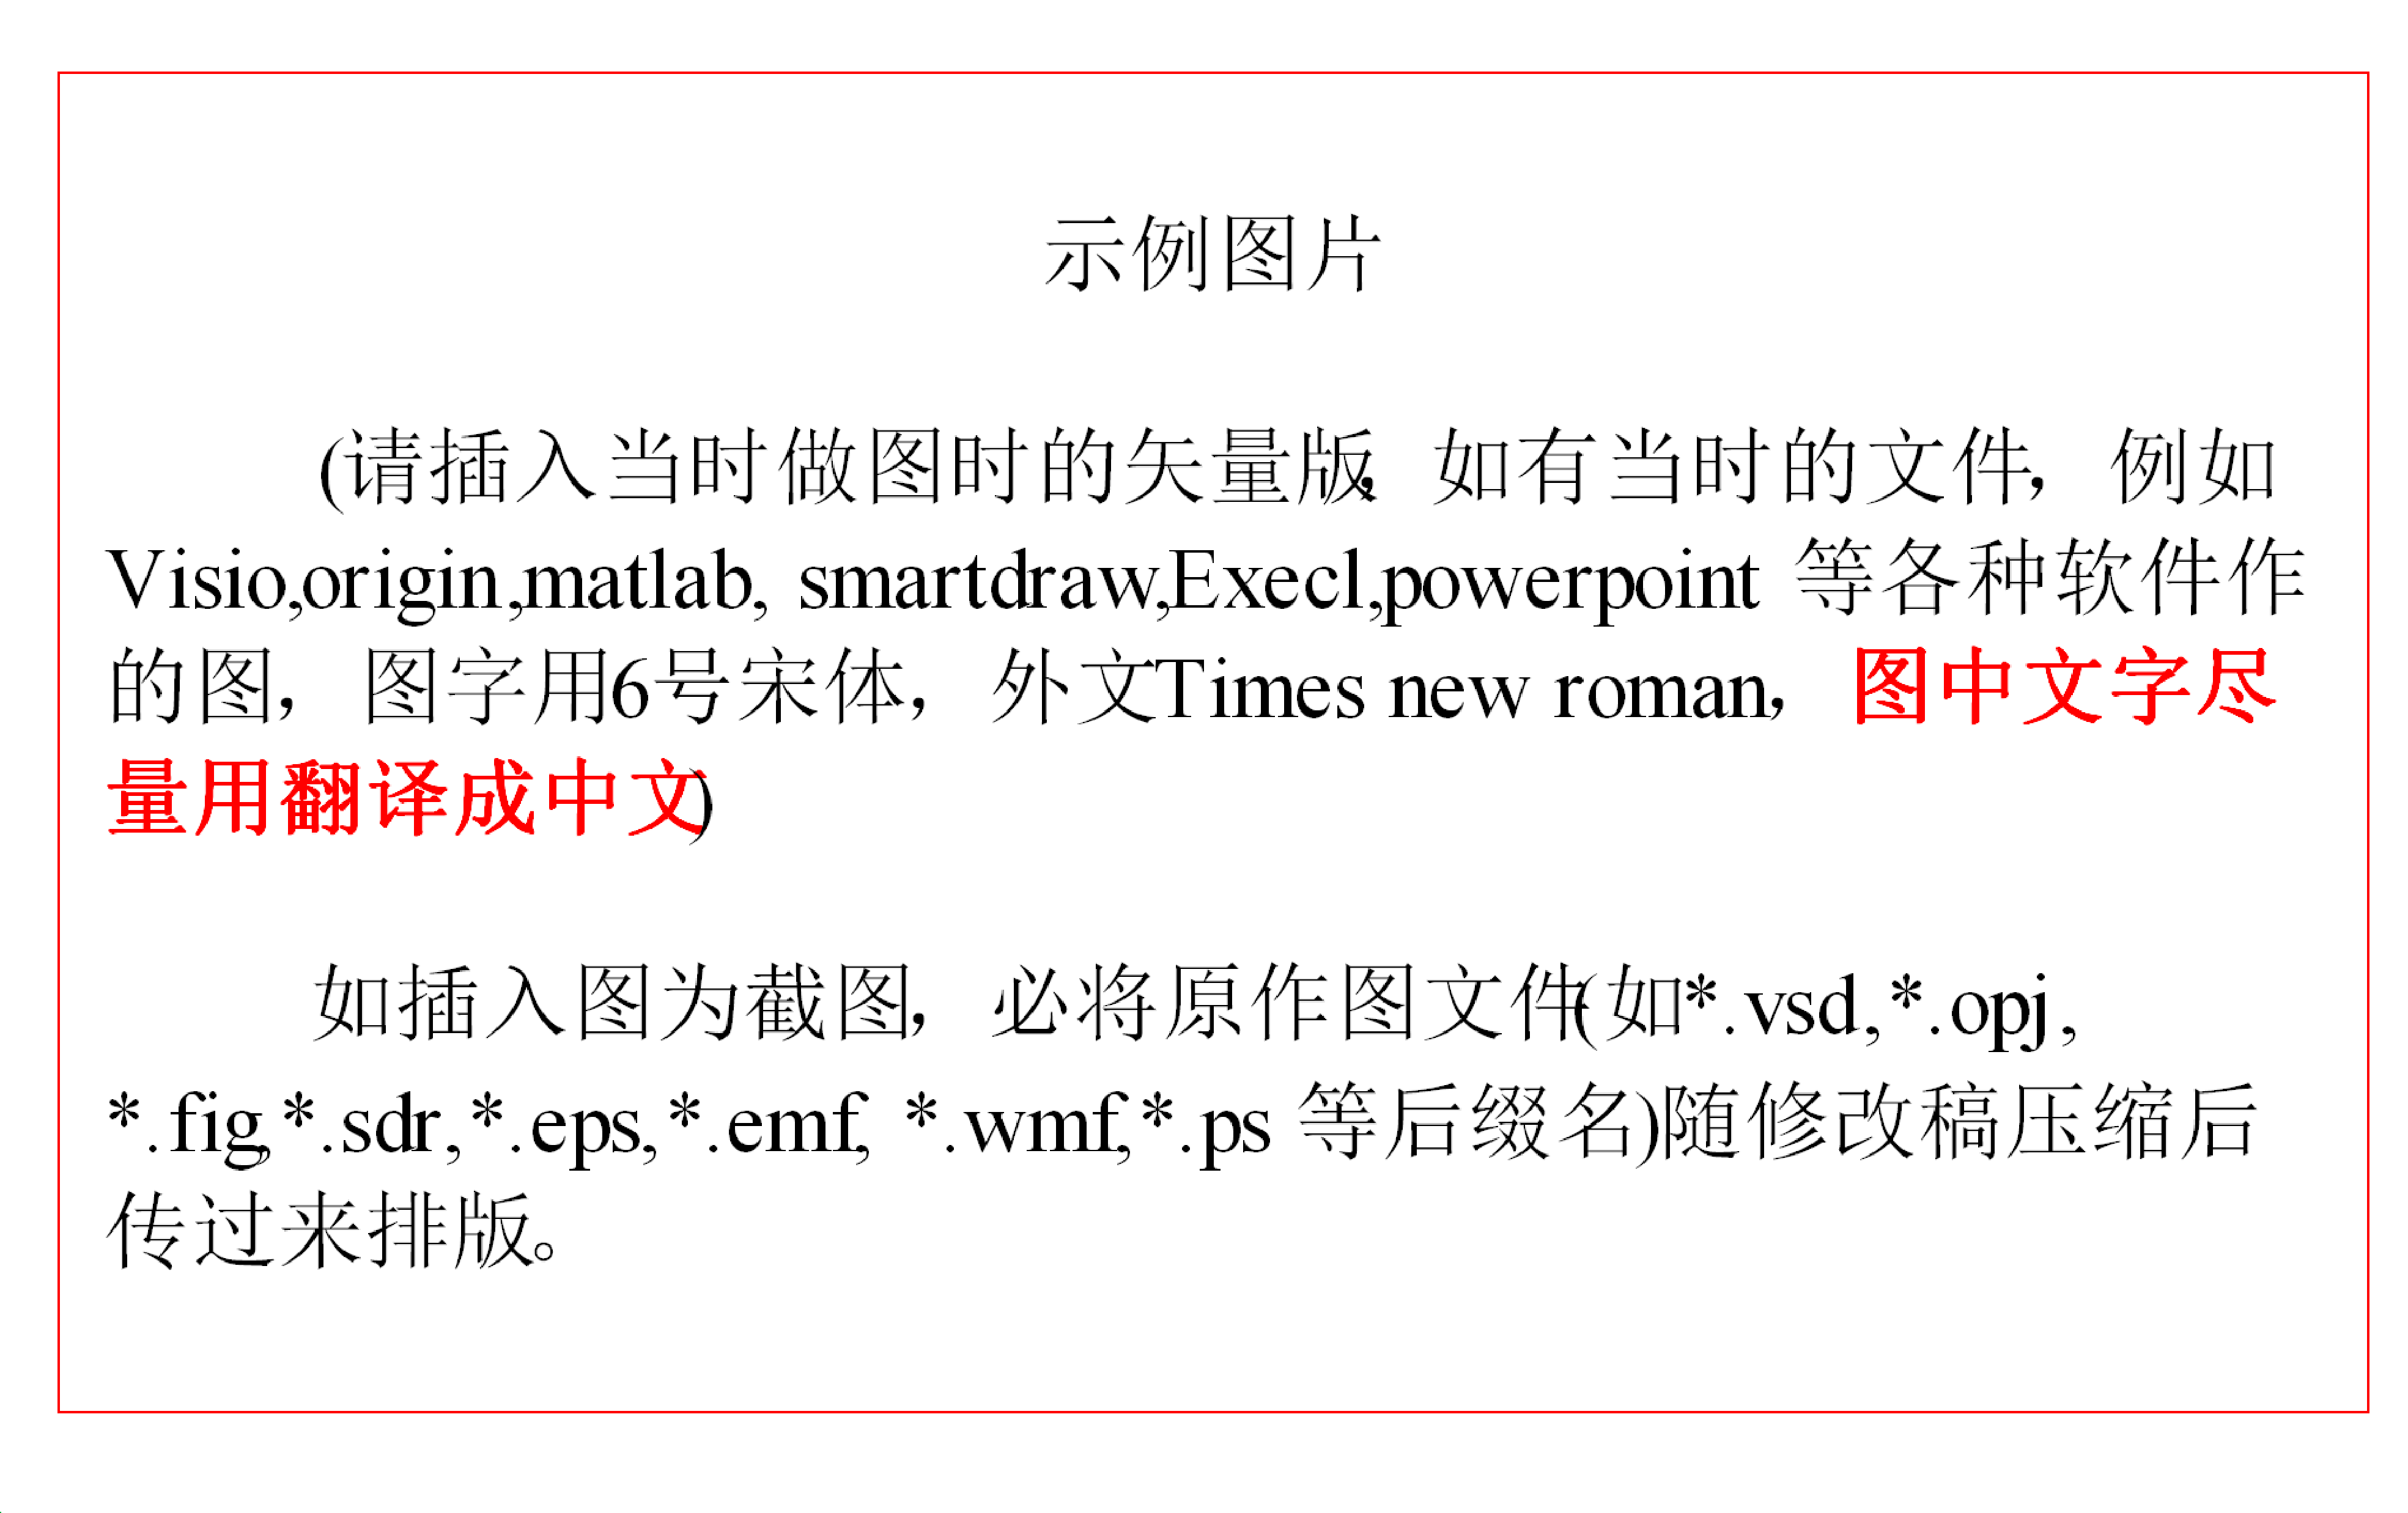
\includegraphics[width=3.15in,height=1.98in]{CJC1.pdf}}
% 图X\quad  图片说明 *字体为小5号，图片应为黑白图，图中的子图要有子图说明*
% \label{CJC1}
% \end{figure}

% \begin{table}[htbp]
% \centering {\begin{CJK*}{UTF8}{zhhei}表X\quad 表说明 *表说明采用黑体*\end{CJK*}}
% \vspace {-2.5mm}
% \begin{center}
% \begin{tabular}{ll}
% \toprule
% *示例表格*&*第1行为表头,表头要有内容* \\
% \hline
% &
%  \\
% &
%  \\
% &
%  \\
% &
%  \\
% \bottomrule
% \end{tabular}
% \label{tab1}
% \end{center}
% \end{table}

% \begin{CJK*}{UTF8}{zhhei}过程X.\end{CJK*}\quad 过程名称

% {\zihao{5-}*《计算机学报》的方法过程描述字体为小5号宋体，IF、THEN等伪代码关键词全部用大写字母，变量和函数名称用斜体*}


% \begin{CJK*}{UTF8}{zhhei}算法\textbf{Y}\end{CJK*}.\quad 算法名称.
% \zihao{5-}{

% \noindent 输入：{\ldots} {\ldots}

% \noindent 输出：{\ldots} {\ldots}

% *《计算机学报》的算法描述字体为小5号宋体, IF、THEN等伪代码关键词全部用大写字母，变量和函数名称用斜体*}

\vspace {3mm}
\zihao{5}{
\noindent \begin{CJK*}{UTF8}{zhhei}致\quad 谢\end{CJK*}\quad \begin{CJK*}{UTF8}{kai}
本项目得以顺利完成, 离不开指导老师的耐心指导与宝贵建议.
在整个开发与撰写过程中, 老师在算法设计思路、技术实现细节及报告规范性方面都给予了我们极大的帮助.

同时, 感谢团队成员在项目中通力合作、分工明确,
特别是在迷宫生成、路径规划、策略优化、图形可视化等模块中的共同攻关与调试, 使得项目功能得以完整实现.

此外, 感谢各类开源资源与社区文档为项目提供了良好的参考与支持,
包括~OpenGL~图形库、SHA-256~加密库及~JSON~解析工具等, 为实现各模块功能提供了重要保障.

再次感谢所有支持和帮助本项目顺利完成的老师与同学们!

\end{CJK*}}


\vspace {5mm}
\centerline
{\zihao{5}
\begin{CJK*}{UTF8}{zhhei}参~考~文~献\end{CJK*}}

\begin{thebibliography}{99}
\zihao{5-} \addtolength{\itemsep}{-1em}
\vspace {1.5mm}

\bibitem[1]{1} Three maze generation algorithms: Depth-First Search, Randomized Prim’s Algorithm, and Recursive Division. \url{https://blog.csdn.net/qq_41517936/article/details/107047349}, 2020-06-30 \newline
(三种迷宫算法（深度优先、随机Prim、递归分割）. \url{https://blog.csdn.net/qq_41517936/article/details/107047349}, 2020年6月30日)

\bibitem[2]{2} Wang Xiao-Dong. Design and Analysis of Computer Algorithms. 5th ed. Beijing: Publishing House of Electronics Industry, 2018 (in Chinese) \newline
(王晓东. 计算机算法设计与分析. 第5版. 北京: 电子工业出版社, 2018)

\bibitem[3]{3} Cormen T. H., Leiserson C. E., Rivest R. L., Stein C. Introduction to Algorithms. 3rd ed. Cambridge, MA: MIT Press, 2009

\bibitem[4]{4} Aho A. V., Hopcroft J. E., Ullman J. D. The Design and Analysis of Computer Algorithms. Boston, MA: Pearson Education, 2007

\bibitem[5]{5} Tree-shaped Dynamic Programming (Tree DP). \url{https://zhuanlan.zhihu.com/p/657528677}, 2023-09-21 \newline
([树形~DP]树形~DP 的通用思路. \url{https://zhuanlan.zhihu.com/p/657528677}, 2023年9月21日)



% \bibitem[1]{1}
% 网上的文献(举例：The Cooperative
% Association for Internet Data Analysis(CAIDA),http://www.caida.org/data
% 2010,7,18) \textbf{*请采用脚注放于正文出现处，每页的脚注从1开始编序号*}
% % \footnote{The Cooperative Association for Internet Data
% % Analysis (CAIDA), http://www.caida.org/data 2010, 7, 18}

% \bibitem[2]{2} 中文的参考文献需给出中英文对照。形式如[3]。

% \bibitem[3]{3} Zhou Yong-Bin, Feng Deng-Guo. Design and analysis of cryptographic
% protocols for RFID. Chinese Journal of Computers, 2006, 29(4): 581-589 (in
% Chinese) \newline
% (周永彬, 冯登国. RFID安全协议的设计与分析. 计算机学报, 2006, 29(4): 581-589)

% \bibitem[4]{4} 期刊、会议、书籍名称不能用缩写。

% \bibitem[5]{5} 作者(外国人姓在前，名在后可缩写, 后同).
% 题目(英文题目第一字母大写，其它均小写)：副标题(如果有). 刊名(全称), 年,
% 卷(期): 页码 \textbf{*期刊论文格式*}

% \bibitem[6]{6}作者.
% 文章题目(英文题目第1字母大写，其它均小写)：副标题(如果有)//Proceedings of
% the {\ldots} (会议名称). 会议召开城市, 会议召开城市所在国家, 年: 页码
% \textbf{*会议论文集论文格式*}

% \bibitem[7]{7}作者. 文章题目(英文题目第一字母大写, 其它均小写):
% 副标题(如果有)//编者. 文集标题. 出版地: 出版社, 出版年: 页码
% \textbf{*文集格式*}

% \bibitem[8]{8}作者. 书名: 副标题(如果有). 版次(初版不写). 出版社地点: 出版社,
% 出版年 \textbf{*书籍格式*}

% \bibitem[9]{9}作者. 文章题目[博士学位论文/硕士学位论文]. 单位名称,单位地点, 年
% \textbf{*学位论文格式*}

% \bibitem[10]{10}作者. 文章题目(英文题目第一字母大写，其它均小写). 单位地点: 单位,
% 技术报告: 报告编号, 年 \textbf{*技术报告*}

% \bibitem[11]{11}专利拥有人. 专利名称，专利授权国家，专利授权日期
% \textbf{*技术专利*}
\end{thebibliography}

  
% \clearpage

\begin{strip}
\end{strip}


\vskip 100mm
\noindent {\zihao{5}\bf{附录~1}. 伪代码}


\begin{algorithm}
\caption{Maze Generation}
\begin{algorithmic}[1]
\Function{genMaze}{$n$}
    \State Initialize maze $M$ with walls
    \State Set entrance and exit on $M$ boundary
    \State $P \gets \emptyset$
    \State $r \gets \frac{n+1}{2}$
    \State \Call{getPath}{$P, 0,0,r-2,r-2$}
    \State \Call{destroyWall}{$P,M$}
    \State \Call{generateElements}{$M$}
    \State \Return $M$
\EndFunction

\Function{getPath}{$P,x_1,y_1,x_2,y_2$}
    \If{$x_1 = x_2$}
        \For{$i=y_1$ \textbf{to} $y_2-1$}
            \State $P \gets P \cup \{((x_1,i),(x_1,i+1))\}$
        \EndFor
        \State \Return
    \EndIf
    \If{$y_1 = y_2$}
        \For{$i=x_1$ \textbf{to} $x_2-1$}
            \State $P \gets P \cup \{((i,y_1),(i+1,y_1))\}$
        \EndFor
        \State \Return
    \EndIf
    \State Choose random $d_i \in [x_1,x_2-1]$, $d_j \in [y_1,y_2-1]$
    \State Open doors around $(d_i,d_j)$, add to $P$
    \State \Call{getPath}{$P,x_1,y_1,d_i,d_j$}
    \State \Call{getPath}{$P,d_i+1,y_1,x_2,d_j$}
    \State \Call{getPath}{$P,d_i+1,d_j+1,x_2,y_2$}
    \State \Call{getPath}{$P,x_1,d_j+1,d_i,y_2$}
\EndFunction

\Function{destroyWall}{$P,M$}
    \ForAll{$e=((x_1,y_1),(x_2,y_2)) \in P$}
        \If{$x_1 = x_2$}
            \State Remove vertical wall between points in $M$
        \Else
            \State Remove horizontal wall between points in $M$
        \EndIf
    \EndFor
\EndFunction

\Function{generateElements}{$M$}
    \ForAll{empty cell $c$}
        \State Place boss, locker, trap, resource with given probabilities
    \EndFor
\EndFunction
\end{algorithmic}
\end{algorithm}


% @ code DP
\begin{algorithm}
\caption{Tree-Based Resource Collection via DFS and DP}
\begin{algorithmic}[2]
\Function{treeDP}{$maze$}
    \State $must[x][y] \gets \textbf{true}$ if node is on path to end
    \State $f[x][y] \gets$ maximum resource from subtree rooted at $(x,y)$
    \Function{DFS}{$x, y, lastx, lasty$}
        \If{$(x,y)$ is end}
            \State $must[x][y] \gets \textbf{true}$; \Return
        \EndIf
        \State $f[x][y] \gets \text{value at } (x,y)$
        \ForAll{neighbor $(u,v)$ of $(x,y)$}
            \If{$(u,v)$ is accessible and $(u,v) \ne (lastx, lasty)$}
                \State \Call{DFS}{$u,v,x,y$}
                \If{$must[u][v]$}
                    \State $must[x][y] \gets \textbf{true}$
                    \State $f[x][y] \gets f[x][y] + f[u][v]$
                \EndIf
            \EndIf
        \EndFor
        \ForAll{non-must neighbor $(u,v)$}
            \State $f[x][y] \gets f[x][y] + \max(0, f[u][v])$
        \EndFor
    \EndFunction
    \State \Call{DFS}{$start_x, start_y, -1, -1$}
    \State \Call{genPath}{$start_x, start_y, -1, -1$} \Comment{Recover actual path}
    \State \Return \textbf{true}
\EndFunction
\end{algorithmic}
\end{algorithm}

\begin{algorithm}
\caption{Path Reconstruction Based on DP Result}
\begin{algorithmic}[3]
\Function{genPath}{$x, y, lastx, lasty$}
    \State Append $(x,y)$ to path
    \If{$must[x][y]$}
        \ForAll{non-must neighbor $(u,v)$ with $f[u][v] > 0$}
            \State \Call{genPath}{$u,v,x,y$}; Append $(x,y)$ to path
        \EndFor
        \ForAll{must neighbor $(u,v)$}
            \State \Call{genPath}{$u,v,x,y$}
        \EndFor
    \Else
        \ForAll{non-must neighbor $(u,v)$ with $f[u][v] > 0$}
            \State \Call{genPath}{$u,v,x,y$}; Append $(x,y)$ to path
        \EndFor
    \EndIf
\EndFunction
\end{algorithmic}
\end{algorithm}

\begin{algorithm}
\caption{SmartRunner \texttt{run()} Main Execution Flow}
\begin{algorithmic}[4]
\Function{SmartRunner.run}{}
    \State Initialize \texttt{currentMaze} with unknowns, mark \texttt{isPushed} to false
    \State Locate start position $(x, y)$ where $originMaze[x][y] = S$
    \State \Call{buildTree}{$x, y$} to build DFS tree and depths
    \State Set $currentMaze[i][j] = originMaze[i][j]$ for $i, j \in 3 \times 3$ neighborhood of $(x, y)$
    \State Mark start as pushed, add $(x, y)$ to queue $q$, path, and initial point

    \While{$q$ is not empty}
        \State Select $(tx, ty) \in q$ with highest priority via \Call{less}{$tx, ty, u, v$}
        \State Pop $(tx, ty)$ from $q$, set $x \gets tx$, $y \gets ty$
        \State Add $(x, y)$ to \texttt{point}, add value to $w$
        \If{$(x, y)$ is $E$ and $B, L$ are both found}
            \State \textbf{break}
        \EndIf
        \State Mark $B, L$ if met; mark surroundings as known in $currentMaze$
        \ForAll{adjacent $(tx, ty)$ of $(x, y)$ not yet pushed}
            \State Mark as pushed and add to $q$
        \EndFor
    \EndWhile

    \For{$i = 1$ to $|point| - 1$}
        \State \Call{genPath}{point[i-1], point[i]} and merge into final \texttt{path}
    \EndFor
    \State \Return \texttt{true}
\EndFunction
\end{algorithmic}
\end{algorithm}

\clearpage

\begin{biography}[./figure/zjd.png]
\noindent
\begin{CJK*}{UTF8}{zhhei}张佳栋\end{CJK*}\ \
负责核心算法模块的实现, 包括树形动态规划路径规划、启发式算法等.
同时编写了可视化部分代码.
以及负责汇报和报告的编写.

工作量占比~$40\%$.

\end{biography}

\begin{biography}[./figure/fw.png]
\noindent
\begin{CJK*}{UTF8}{zhhei}方维\end{CJK*}\ \
负责迷宫数据分支法构造与可视化导出, 以及最优路径和得分的保存.同时协助调试和测试完整流程.

工作量占比~$20\%$.
\end{biography}

\begin{biography}[./figure/lxy.png]
\noindent
\begin{CJK*}{UTF8}{zhhei}逯熙钰\end{CJK*}\ \
负责有限视野下的局部路径策略, 设计并实现了基于预期收益的贪心路径选择算法,
提升了实时策略决策的效率与得分表现.

工作量占比~$20\%$.
\end{biography}

\begin{biography}[./figure/jsh.png]
\noindent
\begin{CJK*}{UTF8}{zhhei}姜舜航\end{CJK*}\ \
负责三位密码的回溯求解以及~BOSS~战分支限界法等关键功能.同时协助调试和测试完整流程.

工作量占比~$20\%$.
\end{biography}


% \begin{strip}
% \end{strip}

% \noindent {\zihao{5}\bf{附录~2}. 组员签字}




% \begin{strip}
% \end{strip}

% \noindent {\zihao{5}\bf{附录X}.}
% \zihao{5}
% \noindent \textbf{Background}

% \zihao{5-}\setlength\parindent{2em}
% *\textbf{附录内容}置于此处，字体为小5号宋体。附录内容包括：\textbf{详细的定理证明、公式推导、原始数据}等*



% \begin{biography}[yourphotofilename.jpg]
% \noindent
% \textbf{Second B. Author} *英文作者介绍内容包括：出生年,学位(或目前学历),职称,主要研究领域(\textbf{与中文作者介绍中的研究方向一致})。*
% *字体为小5号Times New Roman*
% \end{biography}
% \begin{strip}
% \end{strip}
% \zihao{5}
% \noindent \textbf{Background}

% \zihao{5-}{
% \setlength\parindent{2em}
% *论文背景介绍为\textbf{英文}，字体为小5号Times New Roman体*

% 论文后面为400单词左右的英文背景介绍。介绍的内容包括：

% 本文研究的问题属于哪一个领域的什么问题。该类问题目前国际上解决到什么程度。

% 本文将问题解决到什么程度。

% 课题所属的项目。

% 项目的意义。

% 本研究群体以往在这个方向上的研究成果。

% 本文的成果是解决大课题中的哪一部分，如果涉及863$\backslash
% $973以及其项目、基金、研究计划，注意这些项目的英文名称应书写正确。}

\end{CJK*}
\end{document}


